% !TEX TS-program = pdflatex
% !TEX encoding = UTF-8 Unicode

% This is a simple template for a LaTeX document using the "article" class.
% See "book", "report", "letter" for other types of document.

\documentclass[11pt]{article} % use larger type; default would be 10pt

\usepackage[utf8]{inputenc} % set input encoding (not needed with XeLaTeX)

%%% Examples of Article customizations
% These packages are optional, depending whether you want the features they provide.
% See the LaTeX Companion or other references for full information.

%%% PAGE DIMENSIONS
\usepackage{geometry} % to change the page dimensions
\geometry{a4paper} % or letterpaper (US) or a5paper or....
% \geometry{margin=2in} % for example, change the margins to 2 inches all round
% \geometry{landscape} % set up the page for landscape
%   read geometry.pdf for detailed page layout information

\usepackage{graphicx} % support the \includegraphics command and options

% \usepackage[parfill]{parskip} % Activate to begin paragraphs with an empty line rather than an indent

%%% PACKAGES
\usepackage{booktabs} % for much better looking tables
\usepackage{array} % for better arrays (eg matrices) in maths
\usepackage{paralist} % very flexible & customizable lists (eg. enumerate/itemize, etc.)
\usepackage{verbatim} % adds environment for commenting out blocks of text & for better verbatim
\usepackage{subfig} % make it possible to include more than one captioned figure/table in a single float
% These packages are all incorporated in the memoir class to one degree or another...

%%% HEADERS & FOOTERS
\usepackage{fancyhdr} % This should be set AFTER setting up the page geometry
\pagestyle{fancy} % options: empty , plain , fancy
\renewcommand{\headrulewidth}{0pt} % customise the layout...
\lhead{}\chead{}\rhead{}
\lfoot{}\cfoot{\thepage}\rfoot{}

%%% SECTION TITLE APPEARANCE
\usepackage{sectsty}
\allsectionsfont{\sffamily\mdseries\upshape} % (See the fntguide.pdf for font help)
% (This matches ConTeXt defaults)

%%% ToC (table of contents) APPEARANCE
\usepackage[nottoc,notlof,notlot]{tocbibind} % Put the bibliography in the ToC
\usepackage[titles,subfigure]{tocloft} % Alter the style of the Table of Contents
\renewcommand{\cftsecfont}{\rmfamily\mdseries\upshape}
\renewcommand{\cftsecpagefont}{\rmfamily\mdseries\upshape} % No bold!

% MATH
\usepackage{graphicx}
\usepackage{subfig}

\usepackage{mathtools}
\usepackage{float}
\usepackage{listings}
%%% END Article customizations

%%% The "real" document content comes below...

\title{Numerical Optimization - Handin 4}
\author{Martin Simon Haugaard - CDL966}
%\date{} % Activate to display a given date or no date (if empty),
         % otherwise the current date is printed 

\begin{document}
\maketitle
\section*{4.1}
The Minimum can be determined by examining the fact that a circle with radius $\Delta$ has the following property:
\begin{gather*}
\Delta^2 = x^2 +y^2
\end{gather*}
Which can be reformulated into
\begin{gather}
\label{new_y}
y = \sqrt(\Delta^2 - x^2)
\end{gather}
Now calculating the Gradient and the Hessian for the given formula for any point, $x$.
\begin{gather*}
\nabla f(x) = \begin{bmatrix}-40 x_1 (x_2 - x_1 ^2) - 2(1-x_1) \\ 20 (x_2 - x_ 1^2)\end{bmatrix}\\
\nabla^2 f(x) = \begin{bmatrix}40(x_2-3x_1^2)+2 & -40x_1 \\ -40x_1 & 20\end{bmatrix}
\end{gather*}
Calculating these for $x_1 = 0, x_2 = -1$
\begin{gather*}
\nabla f(x) = 11 \\
\nabla^2 f(x) = \begin{bmatrix}42 & 0 \\ 0 & 20\end{bmatrix}
\end{gather*}
All of these informations can then be placed into the formula $m_k(p) = f_k + g_k ^ T p + \frac{1}{2} p^T B_k ^p$ which yields the following function
\begin{gather*}
m_k(p) = 11 - 2x - 20y + 21 x^ 2 + 10 y ^2
\end{gather*}
Now substituting in (\ref{new_y}) the final formula becomes:
\begin{gather*} 
m_k(p) = 11 x^2 - 2x  + 11 - 20 * \sqrt{\Delta^2 - x^2} + 10 \Delta^2
\end{gather*}
Using MATLAB's \textit{fminsearch} function, the minimums of the final formula can be determined. And for various $\Delta$ radius from $0<\Delta \leq 2$ Figure~\ref{fig:4_1_1} is given:
\begin{figure}[H]
    \centering
    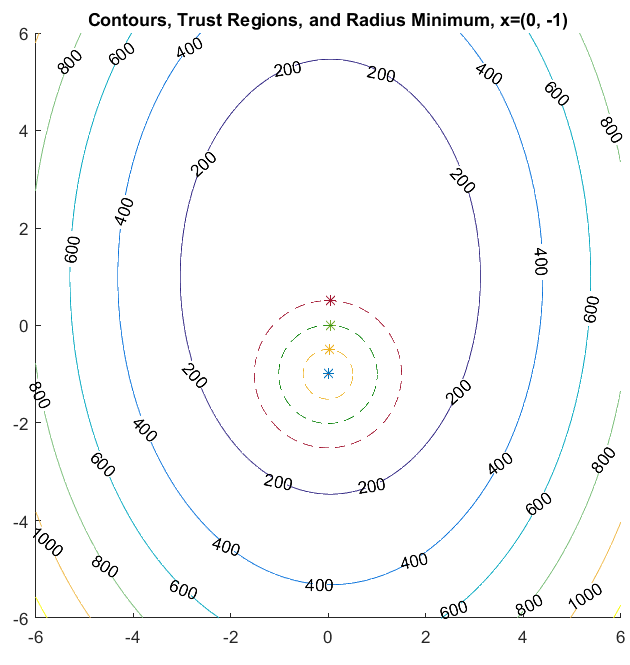
\includegraphics[width=0.5\textwidth]{4_1_1}
    \caption{Contour Lines and Solutions for point $x=(0,-1)$.}
    \label{fig:4_1_1}
\end{figure}
The minimum values seem to make sense, as they all are as close to the minimum of the contour drawing as they can be, while remaining on the trust region border.

\begin{figure}[H]
    \centering
    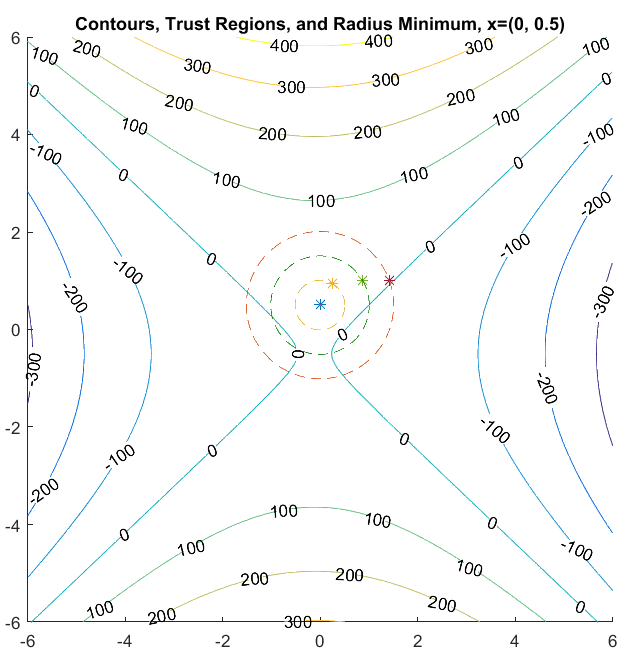
\includegraphics[width=0.5\textwidth]{4_1_2}
    \caption{Contour Lines and Solutions for point $x=(0,0.5)$.}
    \label{fig:4_1_2}
\end{figure}
Following the same steps as with $x=(0,-1)$ the contours for $x=(0,0.5)$ are drawn and once again the (Figure~\ref{fig:4_1_2}).

\section*{4.10}
$B$ is symmetric, that means there can be an orthogonal matrix $Q$ and a diagonal matrix $\Lambda = \{\lambda_1, \lambda_2, \dots \lambda_n\}$, where $\lambda_1 \dots \lambda_n$ are eigenvalues of B for which
\begin{gather*}
B = Q \Lambda Q^T
\end{gather*}

If the lowest of the eigenvalues in $\Lambda$ is greater than or equal to zero, then all the rest of the eigenvalues are also greater than or equal to zero, and then $B$ is positive definite. Which means $B + \lambda I$ is also positive definite, since $ 0 \leq \lambda$.

If the lowest value eigenvalue is negative, then it's possible to choose a $\lambda$ such that it is slightly greater than the absolute value of the lowest eigenvalue. 

Now observing $B = Q \Lambda Q^T$. Doing the calculation $B + \lambda I$ is the same as
\begin{gather*}
B + \lambda I = Q(\Lambda + \lambda I)Q^T
\end{gather*}

Which ensures that the diagonal of $\lambda_1 \dots \lambda_n$ all become positive, since the absolute value of the lowest $\lambda$ in the diagonal is being added to all of them.
Since they are now all positive, the result is positive definite.
\newpage
\section*{Programming Exercise - 4.2}
Implementing the dogleg method, I start with a random $\Delta$ value, lower than the $\hat{\Delta}$, which is the maximum step length. I do the first iteration calculations with this random $\Delta$ value, calculating a $\tau$. Once the $\tau$ is calculated, I calculate the trajectory as described in $(4.16)$. Which I can then use in $(4.3)$ to calculate the next step.
Once I have the next step, I calculate the ratio $\rho$ (4.4), which allows me to scale $\Delta$ as described in \textbf{Algorithm 4.1}. I then update my $x$ and start a new iteration. I terminate the loop once the gradient for the $x$ is sufficiently small, or after a certain (high) amount of iterations.

I plot my iterations as shows in Figure~\ref{fig:dogleg1} \& Figure~\ref{fig:dogleg2}, where I have also plotted the steepest descent method and also newton in Figure~\ref{fig:dogleg1} for comparison.

\begin{figure}[H]
    \centering
    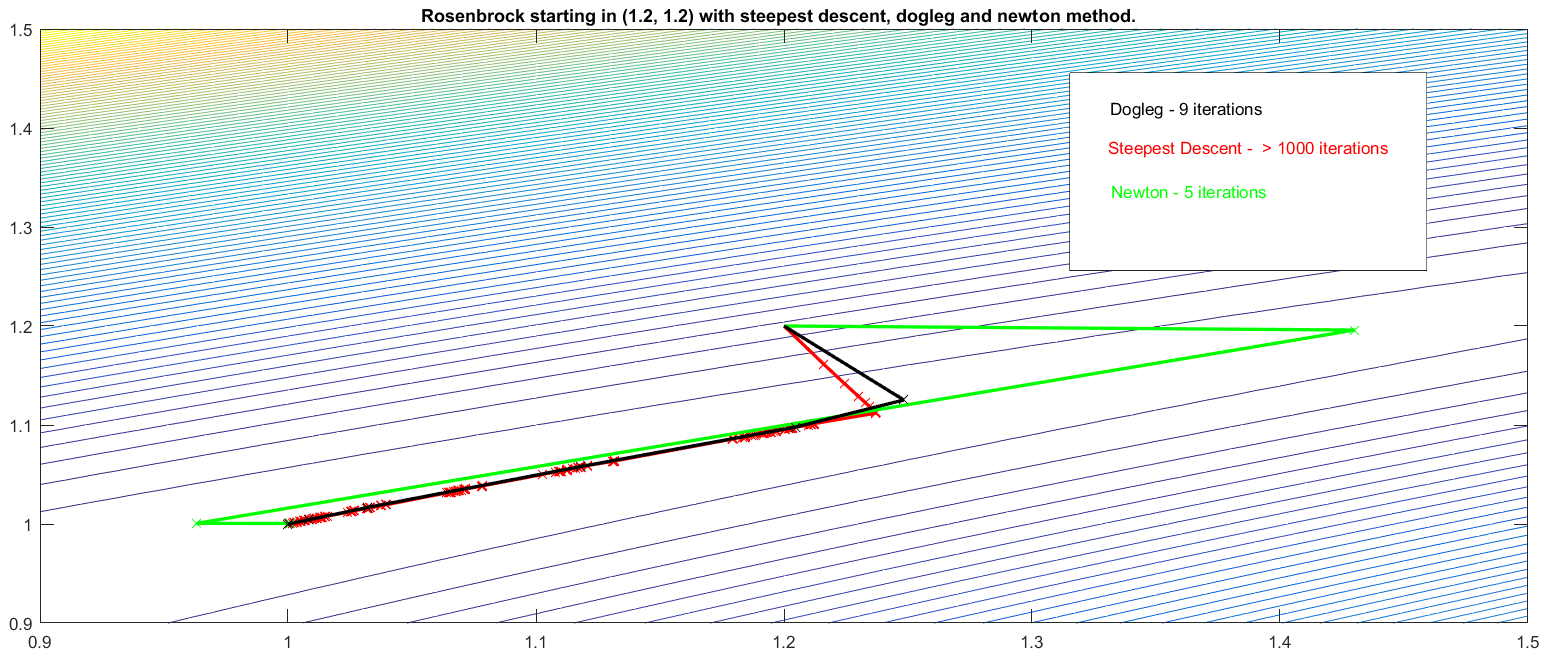
\includegraphics[width=1\textwidth]{12_12_mixed}
    \caption{Steepest Descent, Newton and Dogleg method, starting at $(1.2, 1.2)$}
    \label{fig:dogleg1}
\end{figure}
As noticed last week, the steepest descent will never actually reach the minimum, and it will spend all of it's allowed iterations trying to approach it. Both the Newton and the the dogleg method reaches it fairly quickly however, after 5 and 9 iterations respectively. It's worth noting that the dogleg's approach seems a lot more smooth compared to the newton, as it's almost on top of the steepest descent.

\begin{figure}[H]
    \centering
    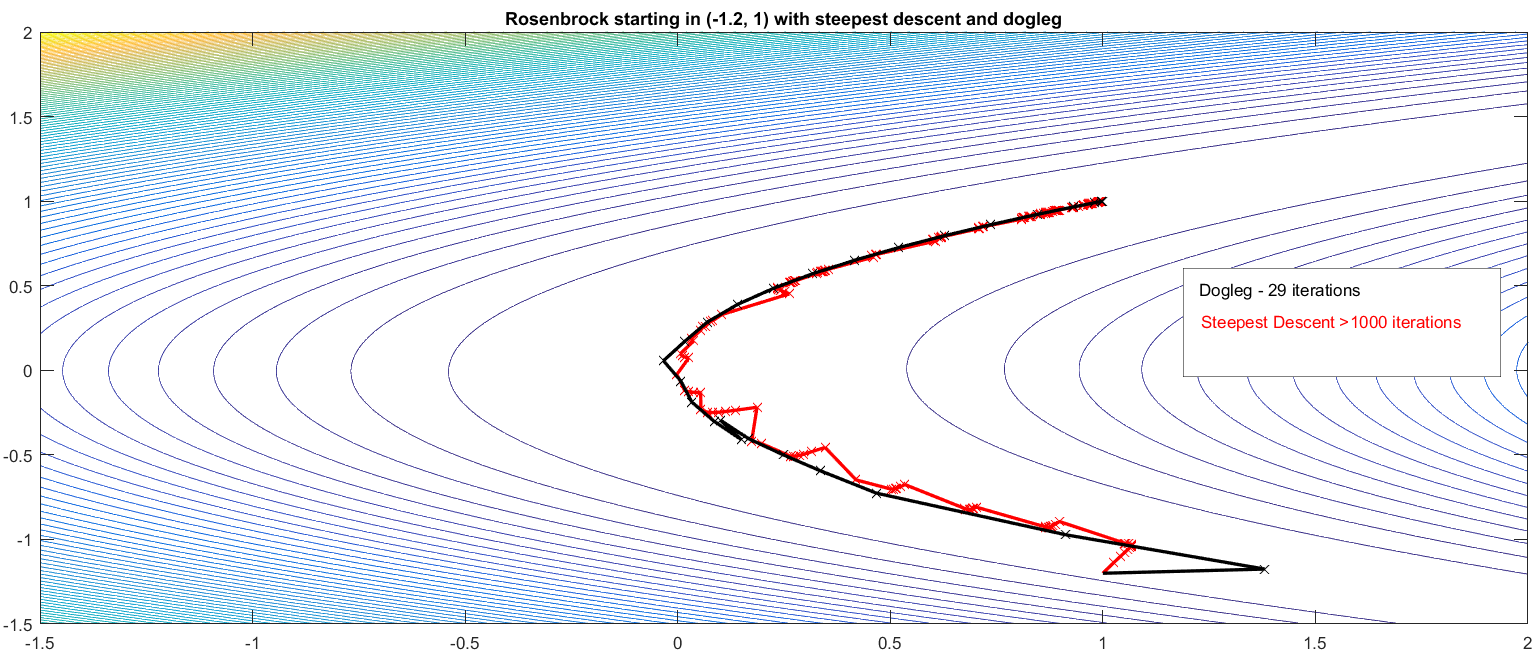
\includegraphics[width=1\textwidth]{-12_1_mixed}
    \caption{Steepest Descent and Dogleg method, starting at $(-1.2, 1)$}
    \label{fig:dogleg2}
\end{figure}
Last week I was unable to make my newton method find the minimum when starting in $x=(-1.2, 1)$ hence it's not included in Figure~\ref{fig:dogleg2}. Once again both the steepest descent and the dogleg approach the minimum, however the steepest descent never gets close enough for a satisfactory gradient. The dogleg does however, after only 29 iterations.

I can conclude that the dogleg method, even with it's slightly more expensive calculations, find the minimum of the rosenbrock function much faster than the steepest descent. I was slightly surprised by the fact that the newton method was four iterations faster than the dogleg in the $x=(1.2, 1.2)$ run. But it seems to make sense, as the descent needed to find the minimum is fairly obvious for $x=(1.2, 1.2)$, hence calculating the dogleg may be too much effort. 
\end{document}
